\documentclass{article}

% Packages
\usepackage[utf8]{inputenc}

\usepackage{amsmath, bm}
\usepackage{graphicx}
\usepackage{amssymb}
\usepackage{float}
\usepackage{caption}
\usepackage{subcaption}
\usepackage{geometry}
\usepackage{multirow}
\usepackage{hyperref}

\newgeometry{vmargin={1in}, hmargin={1in}}


\title{3A1 Transition to Turbulence Lab Report}
\author{[Louis Pender]}
\date{February 29, 2024}

\begin{document}

\maketitle

\section{Introduction}


\section{Objectives}

\begin{itemize}
    \item To observe with the aid of a hot-wire anemometer and a stethoscope the transition
    from a laminar to a turbulent boundary layer on a flat plate:
    \begin{itemize}
        \item when smooth
        \item behind an isolated roughness element on the centre-line of the plate
        \item behind a two-dimensional roughness trip
    \end{itemize}

    \item To obtain the transition Reynolds numbers for the above conditions.
    \item To measure the angle of the turbulent wedge that is formed downstream of the roughness element.
    \item To measure the mean and turbulent profiles of the boundary layer when it is fully turbulent.
    \item To use the mean flow velocity profile to estimate the skin friction co-efficient. % On Clauser Plot
\end{itemize}


\section{Theory}
% Describe the experimental setup, equipment used, and the steps followed during the experiment.

\subsection{Hot wire anemometry}

The hot wire anemometer is a device used to measure the velocity of a fluid.
The wires resistance changes with temperature and the convective heat loss is related to the velocity of the fluid.
This is measured by a Wheatstone bridge circuit which is balanced at a constant temperatue.
The heat loss of the wire can be modelled by King's Law
\begin{equation}
    E^2 = A + B U^{\frac{1}{2}}
\end{equation}
Considering a turbulent flow the velocity profile can be modelled as $\bar{U} + U'$ and similarly, a voltage $\bar{E} + E'$ which represents the sum of a mean value and a fluctuating component.
Additionally the following relation holds:
\begin{equation}
    \frac{E'}{U'} = \frac{d\bar{E}}{d\bar{U}}
\end{equation}
This can be substituted into the King's Law to give
\begin{equation}
    \frac{U'}{E'} = \frac{4\bar{E}\bar{U}^{\frac{1}{2}}}{B} = \frac{4\bar{E}(\bar{E}^2 - A)}{B^2}
    \label{eq:small_kings}
\end{equation}

%%%%%%%%%%%%%%%%%%%%

\section{Results}
% Present the data obtained from the experiment, including tables, graphs, and figures.

The density of air $\rho = 1.225kgm^{-3}$ for the standard atmosphere with 15oC and 760 mmHg
The viscosity of air is $1.7894 \times 10^{-5} Ns/m^2$ at 15oC.

\begin{figure}[H]
    \centering
    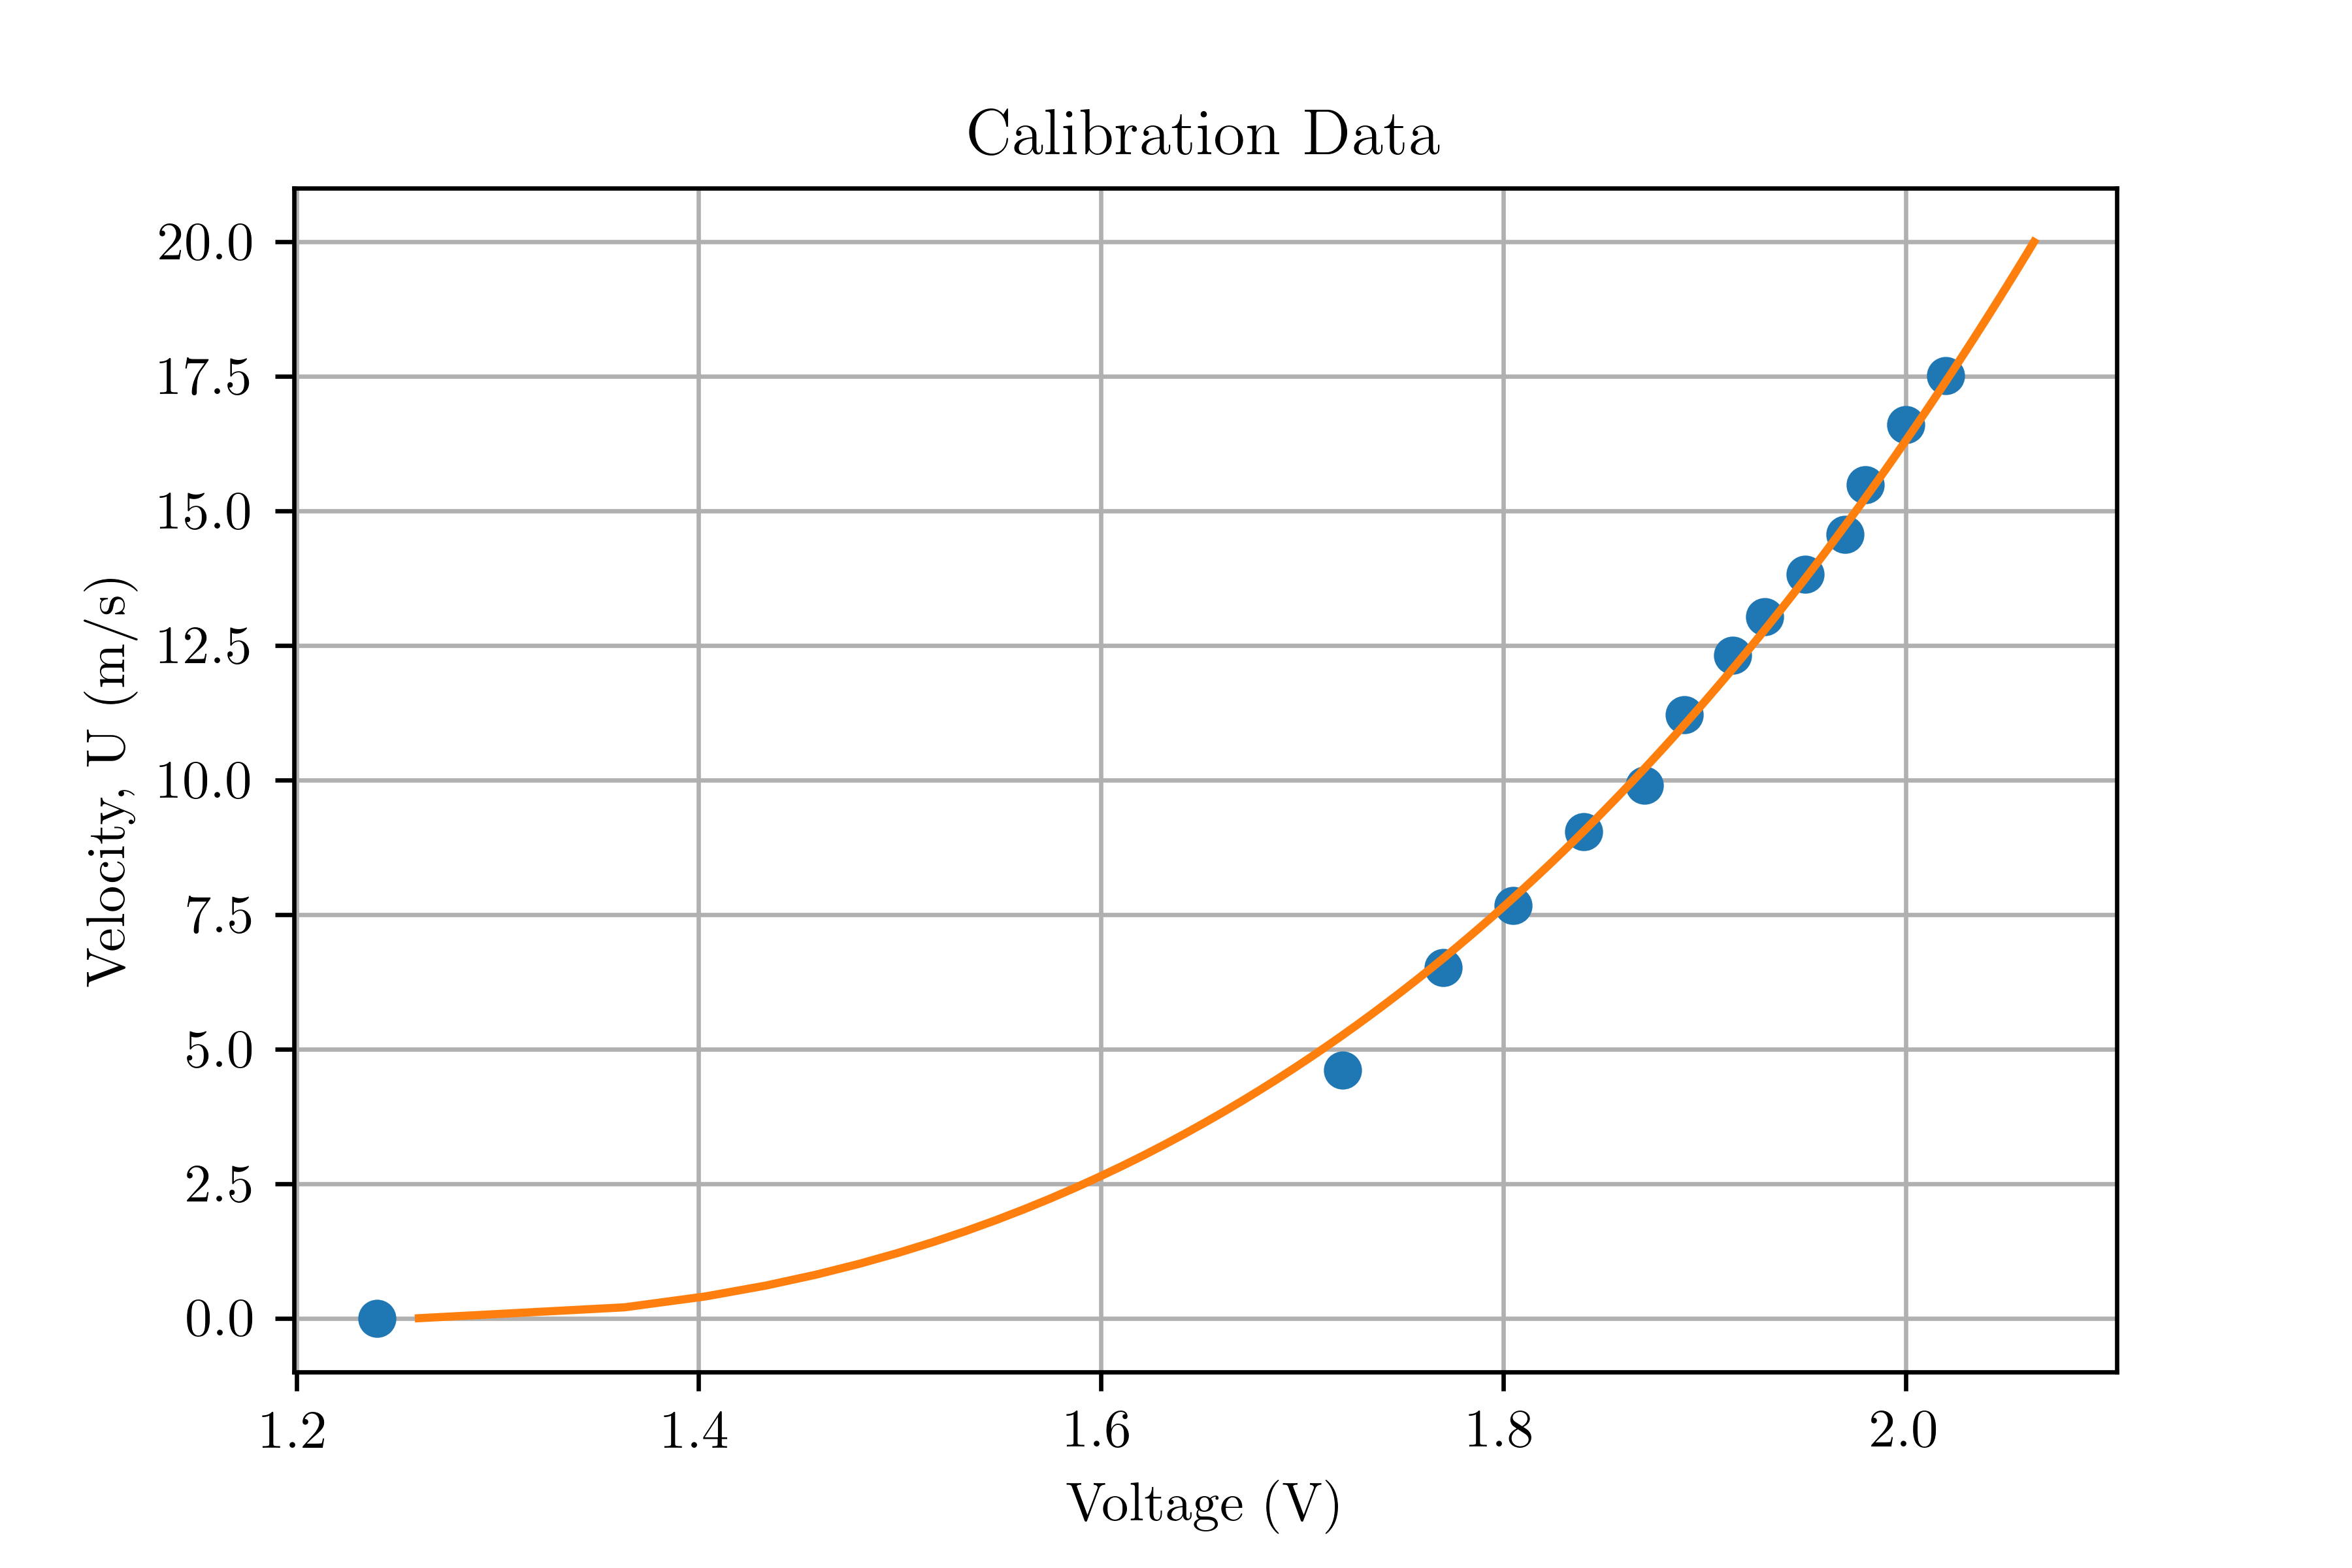
\includegraphics[width=0.8\textwidth]{calibration.png}
    \caption{Calibration curve for the hot wire anemometer}
    \label{fig:calibration}
\end{figure}

\begin{table}[h]
    \centering
    \begin{tabular}{cccccc}
        \hline
        Setup & Dial & $\Delta p$ & $U_{\infty}$ & Re & Comment \\
        & & (mBar) & (m/s) & & \\
        \hline
        \hline
        \multirow{4}{*}{Flat Plate} & 300 & 0.11 & 4.238 & $2.03 \times 10^5$ & Laminar \\
        & 650 & 1.04 &  13.03 & $6.24 \times 10^5$ & Transitioning \\
        & 820 & 1.59 & 16.11 & $7.72 \times 10^5$ & Transitioning \\
        & 1000 & 2.10 & 18.52 & $8.87 \times 10^5$ & Turbulent \\
        \hline
        \hline
        \multirow{3}{*}{Protrusion} & 300 & 0.11 & 4.238 & $2.03 \times 10^5$ & Laminar \\
        & 370 & 0.34 & 7.451  & $3.57 \times 10^5$ & Transitioning \\
        & 430 & 0.47 & 8.760  & $4.20 \times 10^5$ & Turbulent \\
        \hline
        \hline
        \multirow{1}{*}{Trip Wire} & 200 & 0.04 & 2.556 & $1.22 \times 10^4$ & Turbulent \\
        \hline
    \end{tabular}
    \caption{Observations and Reynolds numbers for various arrangements of the tunnel.}
    \label{tab:observations}
\end{table}


\begin{figure}[H]
    \centering 
    \begin{subfigure}{0.8\textwidth}
        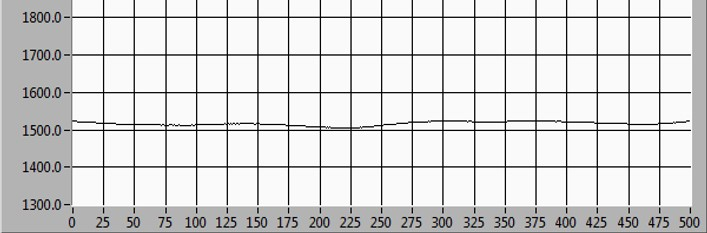
\includegraphics[width=\textwidth]{1_laminar.jpg}
        \caption{Laminar boundary layer at 300 dial}
        \label{fig:oscilloscope_laminar}
    \end{subfigure}
    \begin{subfigure}{0.8\textwidth}
        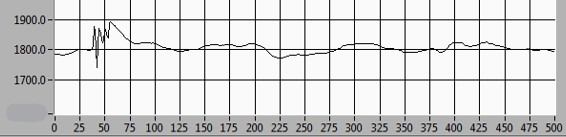
\includegraphics[width=\textwidth]{2_transition.jpg}
        \caption{Transitioning boundary layer at 650 dial}
        \label{fig:oscilloscope_mostly_laminar}
    \end{subfigure}
    \begin{subfigure}{0.8\textwidth}
        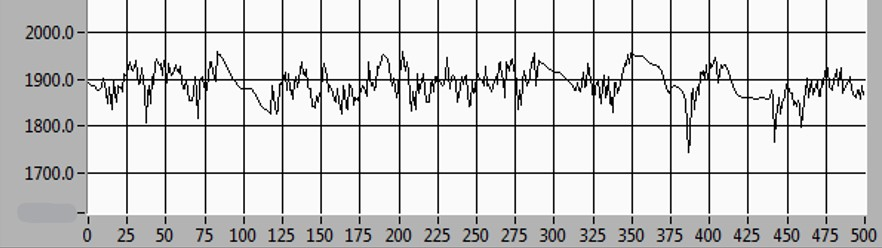
\includegraphics[width=\textwidth]{3_transition.jpg}
        \caption{Transitioning boundary layer at 820 dial}
        \label{fig:oscilloscope_mostly_turbulent}
    \end{subfigure}
    \begin{subfigure}{0.8\textwidth}
        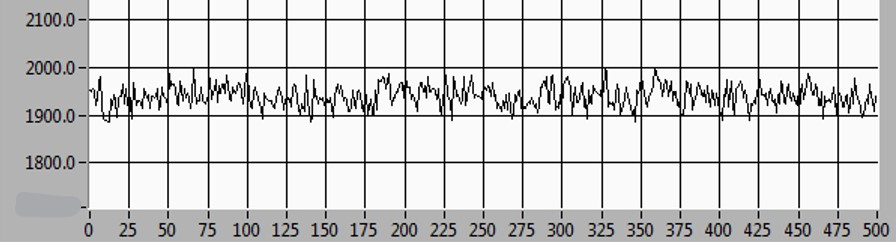
\includegraphics[width=\textwidth]{4_turbulent.jpg}
        \caption{Turbulent boundary layer at 1000 dial}
        \label{fig:oscilloscope_turbulent}
    \end{subfigure}
    \caption{Aenometer oscilloscope readings for various tunnel speeds for the flat plate at a distance of 0.2mm}
    \label{fig:oscilloscope}
\end{figure}

% 1. Express your results in terms of the Reynolds number.

\begin{figure}[H]
    \centering
    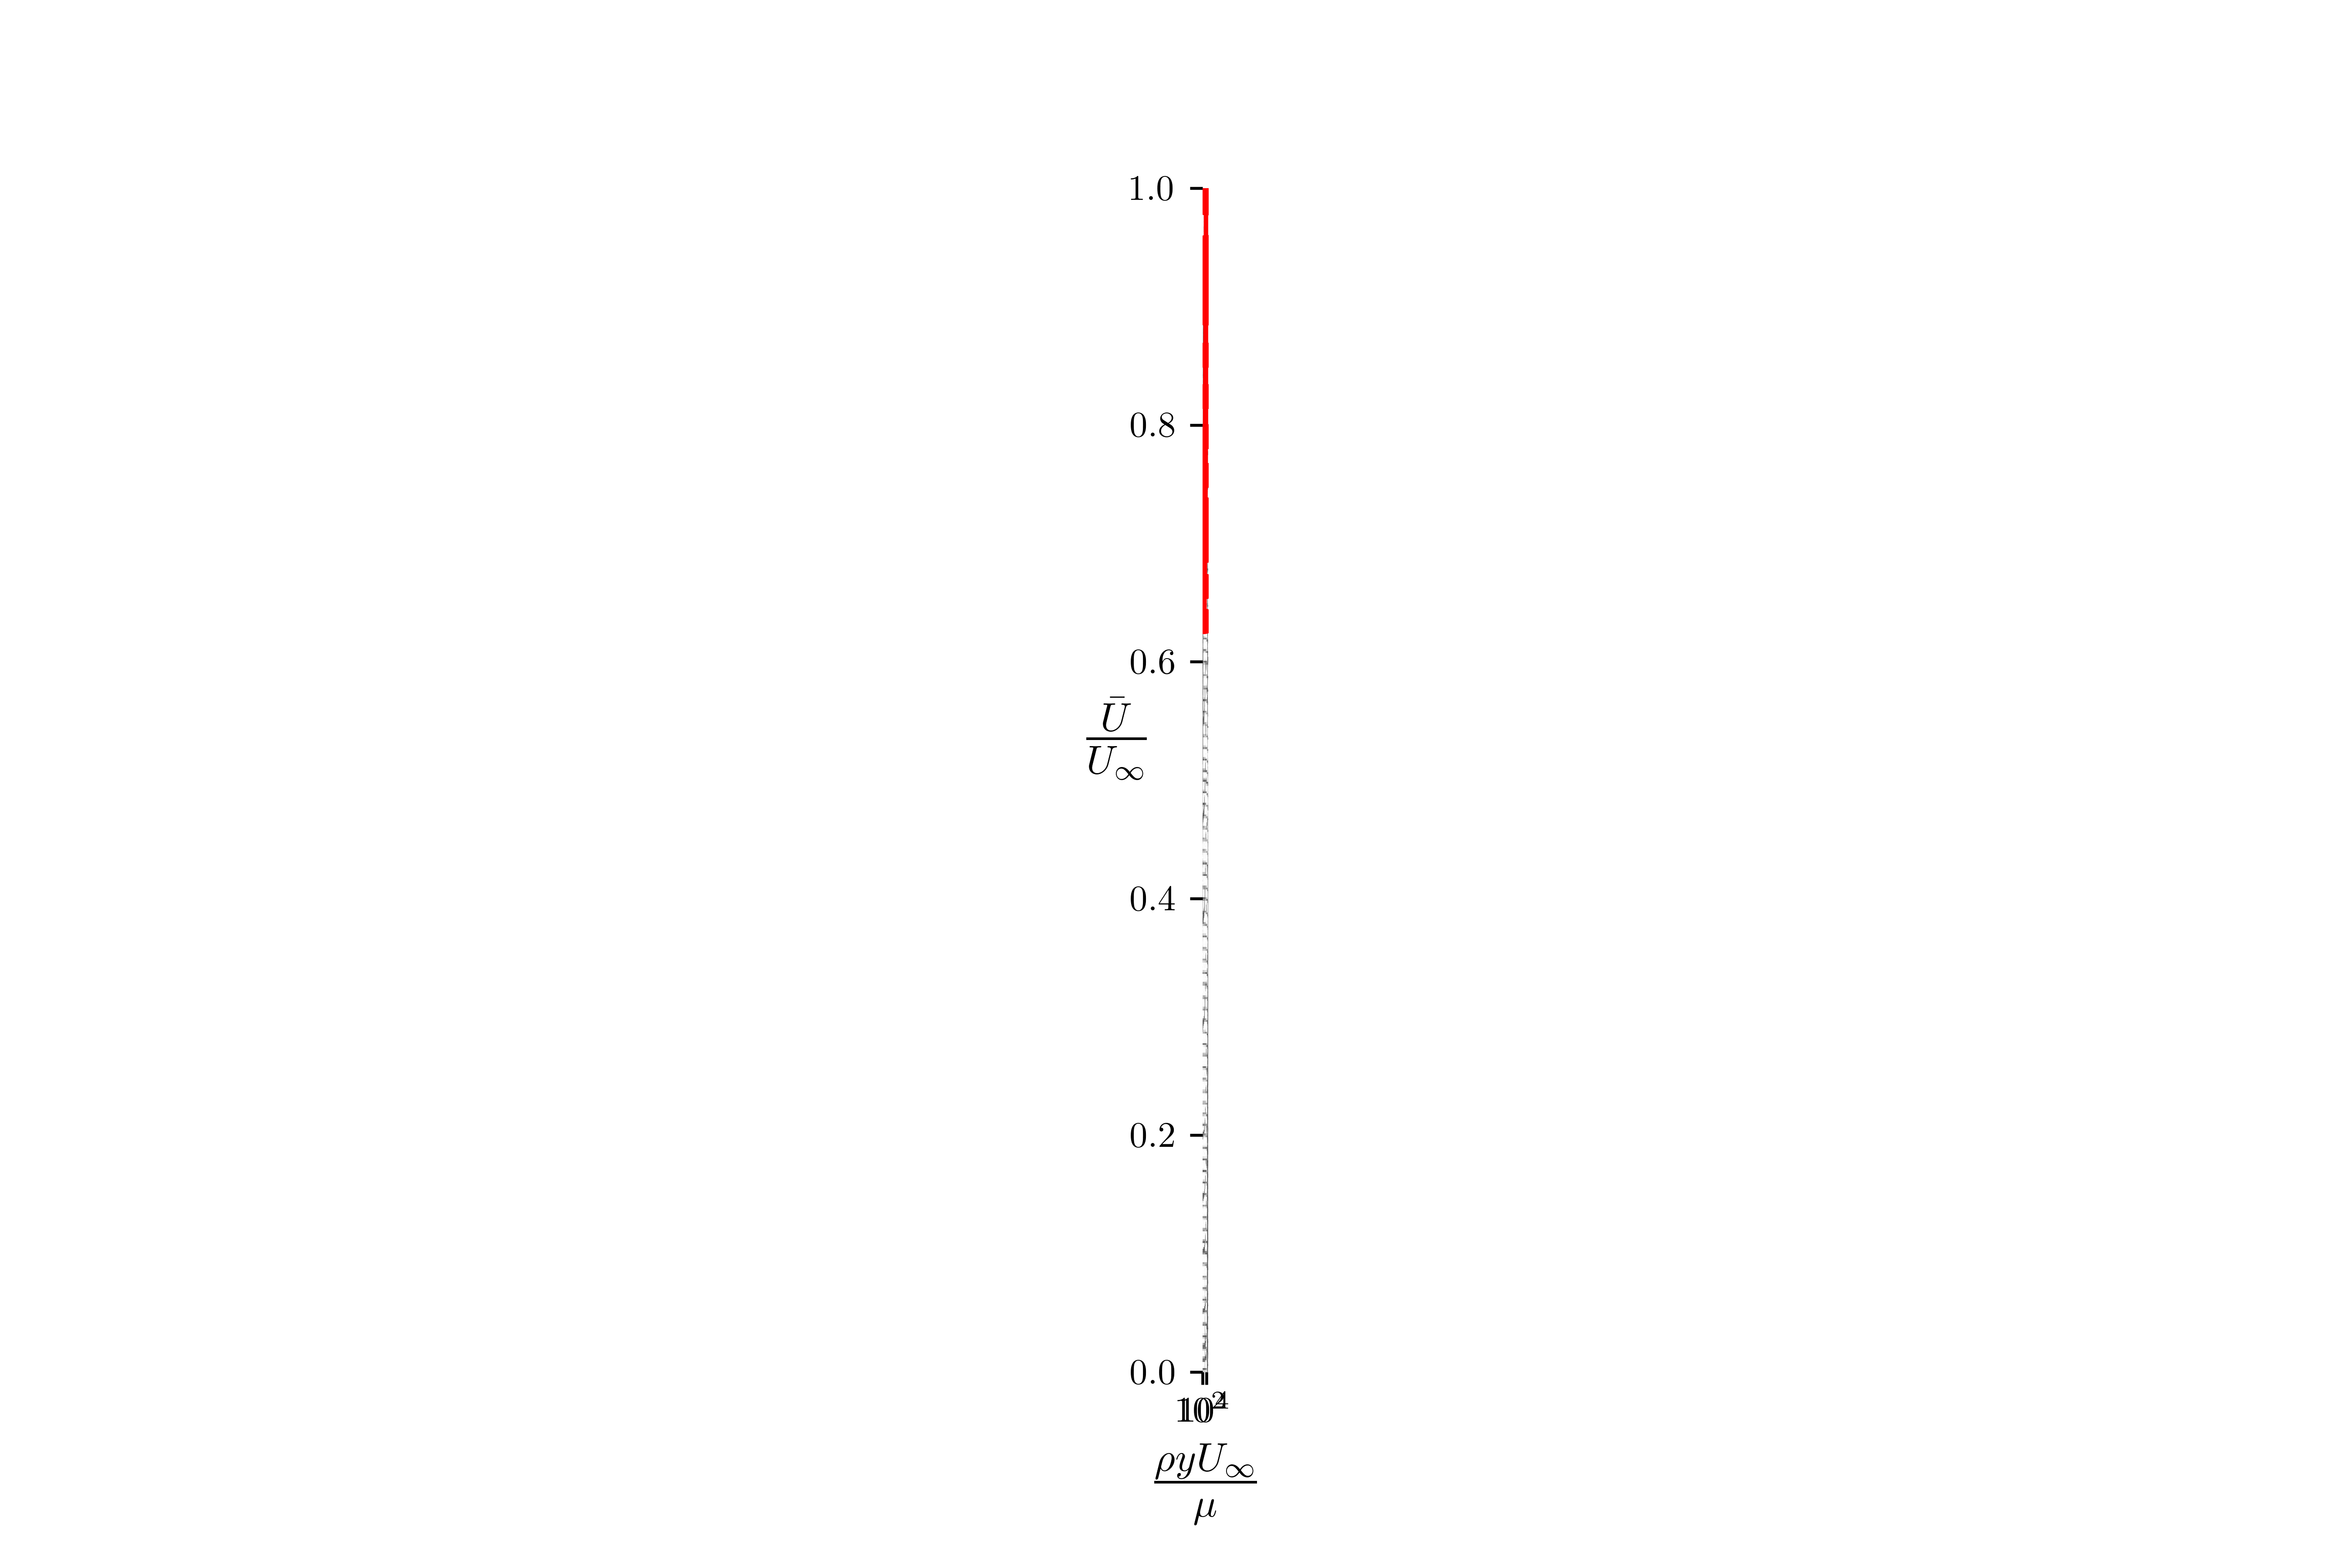
\includegraphics[width=0.99\textwidth]{clauser_data.png}
    \caption{Clauser plot of turbulent boundary layer profile for a dial setting of 500}
    \label{fig:clauser}
\end{figure}

\begin{figure}[H]
    \centering
    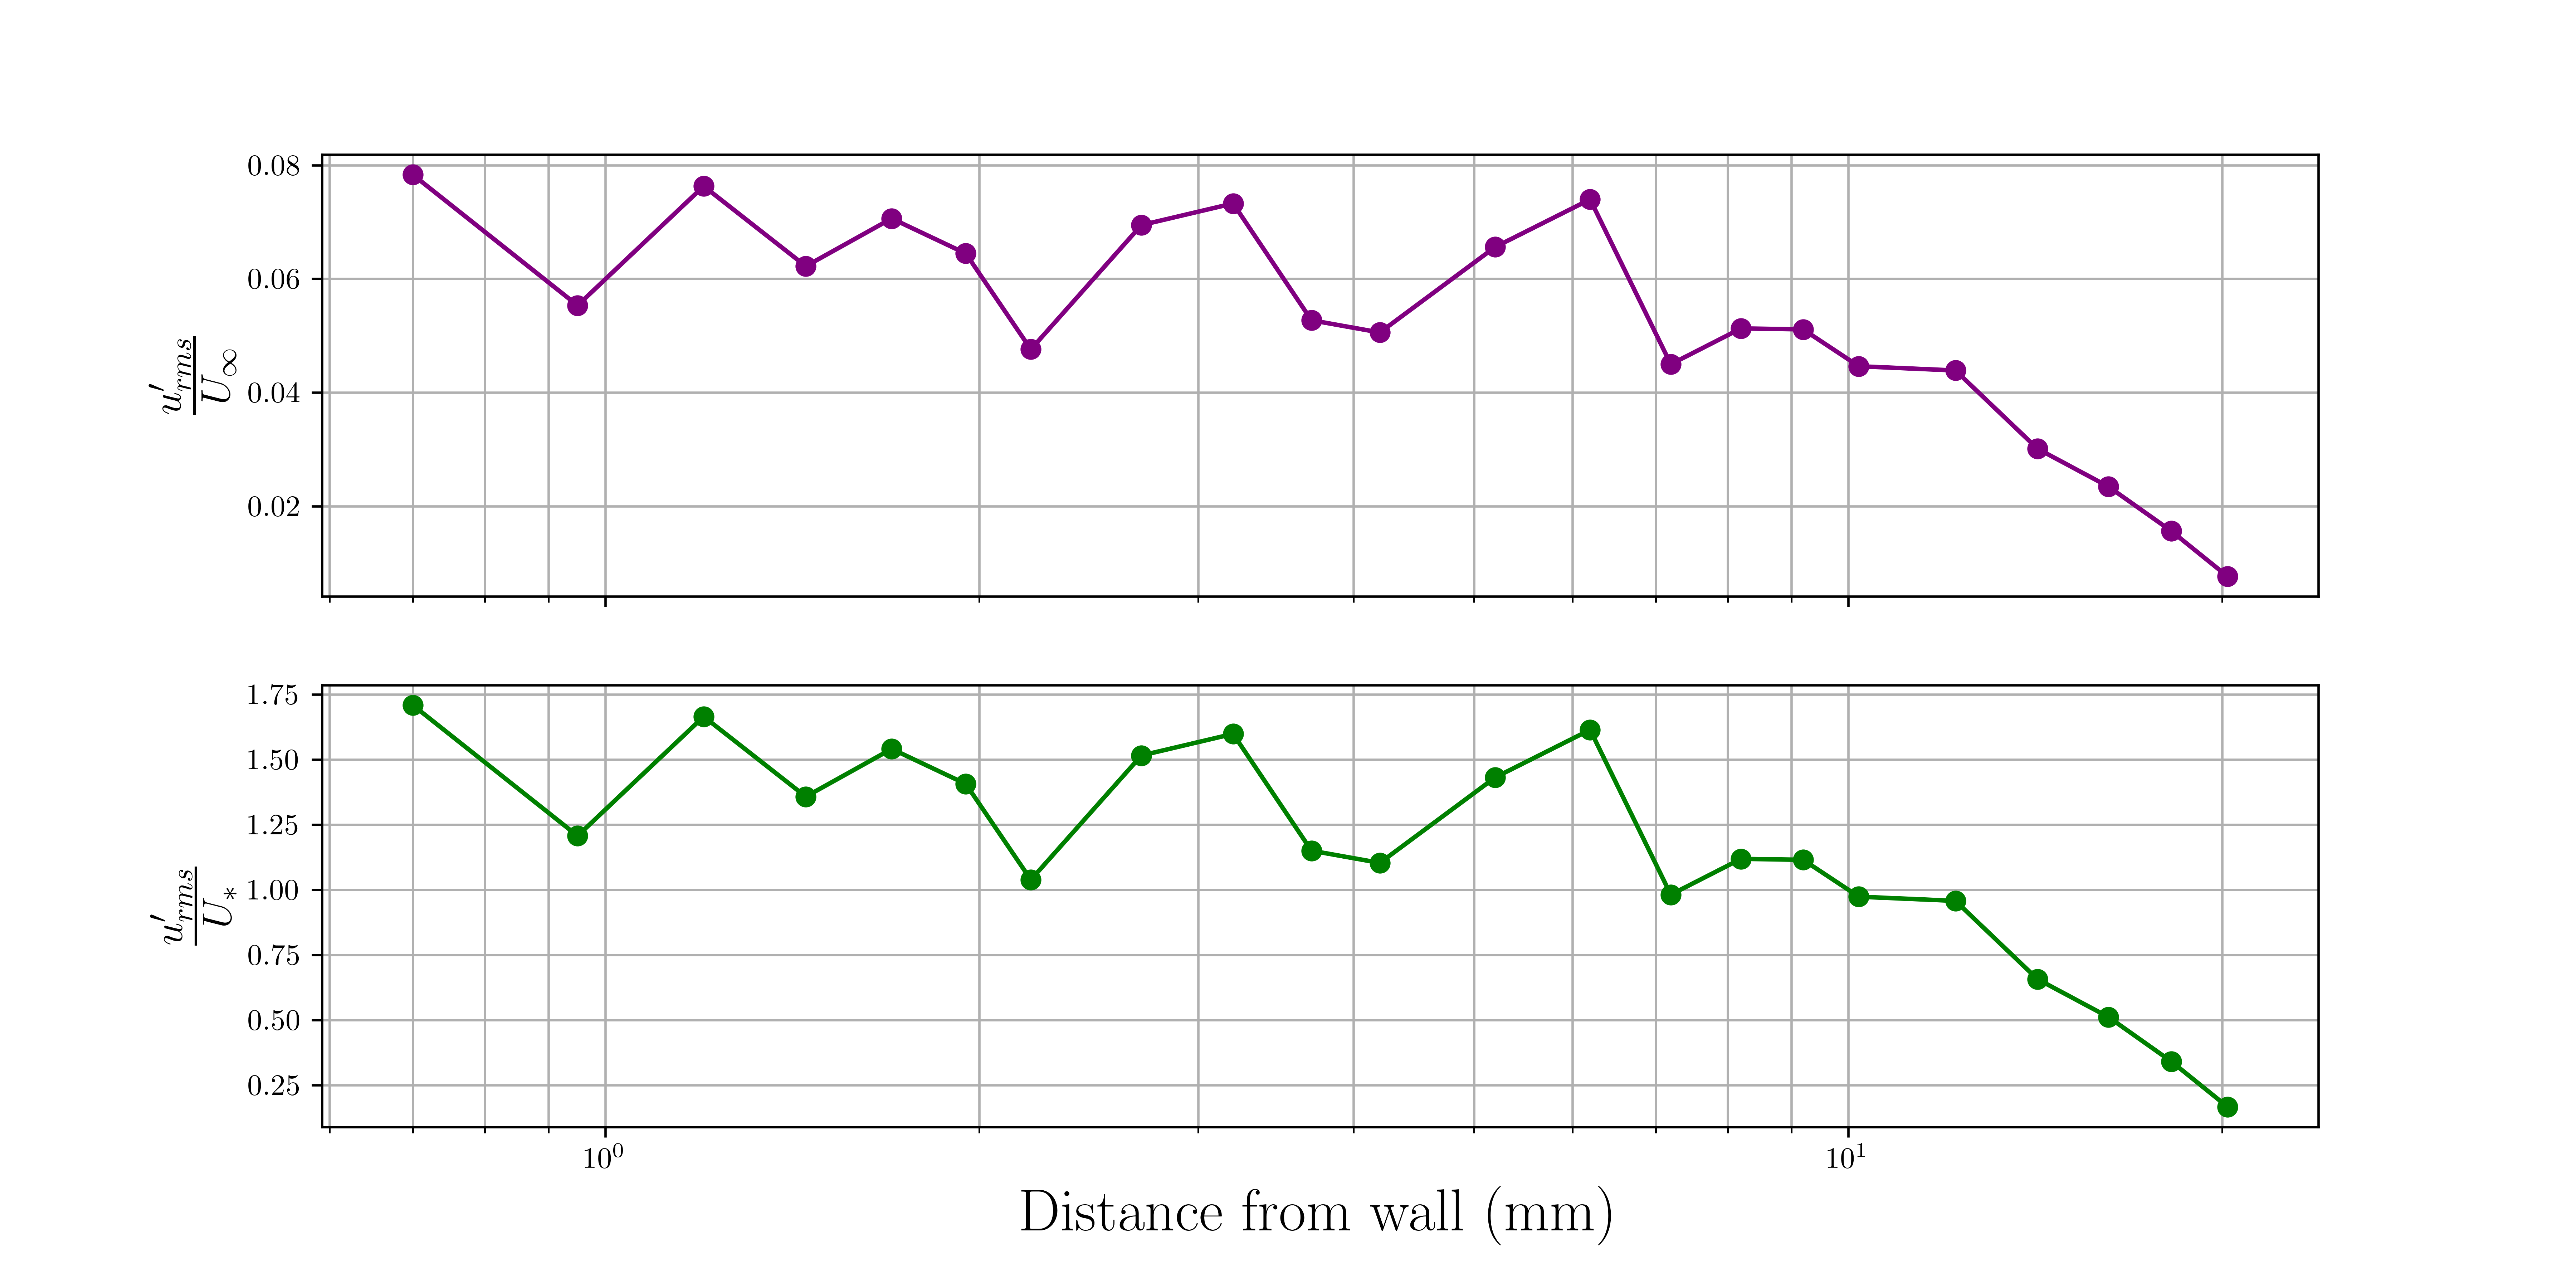
\includegraphics[width=0.99\textwidth]{u_fluctuation.png}
    \caption{Fluctuation of velocity with distance from the wall}
    \label{fig:fluctuation}
\end{figure}

%%%%%%%%%%%%%%%%%%%%%%%

\section{Discussion}
% Analyze and interpret the results, discussing their significance and any observations or trends.
%  laminar skin friction drag is smaller than turbulent skin friction drag, for the same inflow. 


% 2. Discuss the observations you have made.

%%% Kings law agrees with data?
Figure \ref{fig:calibration} shows the calibration curve for the hot wire anemometer.
The data points obtained agree with the model of King's Law, which is a good indication that the anemometer is functioning correctly.
The values for A and B were found as $A	= 1.589867$ and $B	= 0.596894$.

%%% observations of turbulent regions in the boundary layer table 1 and figure 2
%%%

Figure \ref{fig:oscilloscope} shows the oscilloscope readings for the anemometer at various tunnel speeds.
Figure \ref{fig:oscilloscope_laminar} shows a fully laminar boundary layer as the voltage is smooth, 
however upon increasing tunnel speed increased fluctuations in voltage were observed, as seen in figure \ref{fig:oscilloscope_turbulent}.
From equation \ref{eq:small_kings}, this corresponds to fluctuations in velocity, which is an indication of turbulent eddies in the boundary layer.
Table \ref{tab:observations} shows the Reynolds number for the corresponding tunnel speeds.
From literature it is known that the transition Reynolds number for a flat plate is $Re_{\delta} \approx 5 \times 10^5$.
This agrees nicely with observations made, however the actual transition point depends on surface 


%%% Stethoscope observations for the different arangements



% 3. How long are the intermittent patches of turbulence (spots) in the transition zone?
% calcualted from the local velocity and time difference between the spots

% 4. Try to estimate the size of a typical eddy in the turbulent flow.
%% Done by measuring the time between the peaks of the velocity fluctuations and using local fluctuations in velocity

% 5. For the boundary layer profile, calculate the velocity ratio u'/U1
% where u'(y) is the velocity at height y and U1 ( is the free-stream velocity, and plot versus y, the distance
% from the surface. The points should also be plotted on the Clauser plot supplied. The
% demonstrator will provide you with the zero offset when the probe stop is just in
% contact with the plate (≈ 0.2mm).

The boundary layer profile is shown on the Clauser plot in Figure \ref{fig:clauser}.
It can be observed that

From interpolating the between linear regions on the Clauser the skin friction coefficient is estimated to be $C_f = 0.0042$.
The friction velocity is then given by:
\begin{equation}
    U_* = \left( \frac{\tau}{\rho} \right)^{\frac{1}{2}} = \left[ \frac{1}{2}C_f \bar{ U}_1^2 \right]^{\frac{1}{2}}
\end{equation}


% 7. Calculate and plot versus distance from the wall on separate axes and discuss

\section{Conclusion}
% Summarize the main findings of the experiment and draw conclusions based on the results.


%%%%%%%%%%%%%%%%%%%%%%%

\section{Appendix}

\begin{thebibliography}{9}
    \bibitem{handout}
    Cambridge University Engineering Department, \textit{Module 3A1: Transition to Turbulence Lab Handout}
\end{thebibliography}

\end{document}
